\documentclass[11pt]{article}
\usepackage[utf8]{inputenc}
\usepackage[T1]{fontenc}
\usepackage{amsmath}
\usepackage{amsfonts}
\usepackage{amssymb}
\usepackage[version=4]{mhchem}
\usepackage{stmaryrd}
\usepackage{graphicx}
\usepackage[export]{adjustbox}
\graphicspath{ {./images/} }

\begin{document}
Real Estate Development

This session discusses equity participations in real estate investments. Real estate equity investments are residual claims. In other words, the value of an equity investment in real estate is equal to the value of the underlying real estate property minus the value of mortgage claims, if any, against that real estate. The previous session provided detailed information about mortgages. This chapter provides details about the valuation and analysis of the equity claims on real estate and begins with a discussion of real estate development.

Real estate development projects can include one or more stages of creating or improving a real estate project, including the acquisition of raw land, the construction of improvements, and the renovation of existing facilities. The development phase may terminate with the sale of improved parcels to interested buyers or through the leasing of improved properties. Typically, real estate development entails (1) acquiring land or a site; (2) estimating the marketing potential and profitability of the development project; (3) developing a building program and design; (4) procuring the necessary public approvals and permits; (5) raising the necessary financing; (6) building the structure; and (7) leasing, managing, and perhaps eventually selling the property.

\section*{Real Estate Development as Real Options}
This section focuses on issues related to the initial stages of development. Development is one of the most entrepreneurial as well as one of the riskiest sectors in the real estate investment space. The primary risks involved in real estate development center around the possibility that a project will fail to progress successfully into realization of the perceived potential. Two key factors differentiate development projects from standing real estate investments. First, real estate development is a process in which a new asset is being created. Second, during the lifetime of the development, there is a high degree of uncertainty regarding the estimates of the revenues and costs of the investment.

Most real estate development projects may be viewed as a string of real options. A real option is an option on a real asset rather than a financial security. The real option may be a call option to purchase a real asset, a put option to sell a real asset, or an exchange option involving exchange of nonfinancial assets.

Each expenditure in the development process may be viewed as the purchase of a call option. Consider a stylized three-stage real estate project that involves (1) an initial feasibility analysis, (2) the purchase of a suitable tract of land, and (3) the construction of a building, all of which lead to the ownership of a completed project. The potential to move forward with the third stage (after the second stage has been completed) may be viewed as a call option in which the developer has the option to pay money and contribute vacant land in exchange for an improved property. The potential to move forward with the second stage (after the first stage has been completed) may be viewed as a call option in which the developer has the option to pay money to receive vacant land, which is itself an option on further development. The first stage, payment for a feasibility analysis, may be viewed as the purchase of a call option on a call option (the second stage), which is in turn a call option on the final stage.

A view of the stages of real estate development as a string of call options provides intuition into understanding the risks of real estate development. But the option view can also reveal important insights into the value of a project. The following sections illustrate the application of option theory to a simplified real estate development project.

\section*{An Example of a Real Estate Project with Real Options}
Consider a decision of whether to build a large hotel next to a stadium that is trying to obtain a franchise for a major sports team. The project being considered is to be the official hotel of the stadium. The sports league will announce its decision regarding whether to award the franchise in exactly one year. If the sports franchise is granted, the need for the hotel will begin two years later (a total of three years from the present time). To be the official hotel, the hotel must be finished when the games begin. It will take three years to build the hotel. Therefore, any decision to build the hotel must be made now. Assume the following costs to getting the hotel opened:

\begin{center}
\begin{tabular}{|llr|}
\hline
First Year & Purchase of rights, land, plans, and permits & $\$ 10,000,000$ \\
Second Year & Construction of building shell & $\$ 20,000,000$ \\
Third Year & Construction of building interior and furnishings & $\$ 20,000,000$ \\
Total &  & $\$ 50,000,000$ \\
\hline
\end{tabular}
\end{center}

Assume for simplicity that if the sports franchise is successful, the hotel will be a terrific investment worth $\$ 80$ million when it opens. However, if the sports franchise is denied, then the hotel will struggle to attract guests and be worth only $\$ 20$ million. Should the project be begun?

To begin the analysis, assume that there is a 50\% chance that the franchise will be granted, whereby the hotel will be worth $\$ 80$ million, and a $50 \%$ chance that the hotel will be worth only $\$ 20$ million. Using these probabilities, the expected value of the hotel is $\$ 50$ million.

To make the analysis as simple as possible, assume that interest rates are $0 \%$. Thus, the expected value of the hotel and the total cost of the completed project are both $\$ 50$ million, and it would appear that the project would have a zero expected value (i.e., net present value). Ignoring options theory, it appears as though the only way this project would be viable would be if the probability of the franchise being granted were more than $50 \%$.

But this analysis ignores an important real option that exists throughout such construction projects: the right to abandon the project or change plans if events unfold that make the continuation of the existing project undesirable. Ignoring interest rate and other risks, when the option to abandon is included, the sports hotel project should be undertaken even if there is only a $25 \%$ chance of the franchise being granted.

Here's how the abandonment option may be viewed. First, the developer pays $\$ 10$ million for all first-year expenses to acquire the rights, land, plans, and permits. If after that first year the franchise is granted, then the developer has the right to continue the project by building the hotel for another $\$ 40$ million. The investors would then make a $\$ 30$ million profit, since the hotel costs $\$ 50$ million and is worth $\$ 80$ million. On the other hand, if after one year the franchise is denied, the investors would abandon the hotel for a total loss of $\$ 10$ million. In most real situations, some of the investment might be recouped, such as would be the case in this example if the land still had value.

Thus, if there is a $25 \%$ chance that the franchise would be granted, there would be a $75 \%$ chance of losing $\$ 10$ million and a $25 \%$ chance of making $\$ 30$ million, and the project would represent a fair investment. Any higher probability of the franchise being granted would create a positive expected value.

\section*{Decision Trees}
In the sports hotel example, there were two decision points. The first was whether to begin the project, and the second was whether to abandon the project after the first year. In practice, a real estate development project can have numerous decision points at which a project can be terminated or modified. Projects can also be delayed, expanded, reduced, or otherwise altered, such as by devising a change in purpose.

To analyze more complex problems, it is often useful to construct a decision tree. A decision tree (as depicted in the Decision Tree for the Sports Hotel exhibit) shows the various pathways that a decision maker can select, as well as the points at which uncertainty is resolved. A decision tree enables analysis and solutions regarding the choices that should be made based on various decision-making points and on new information as that information becomes available.

\begin{center}
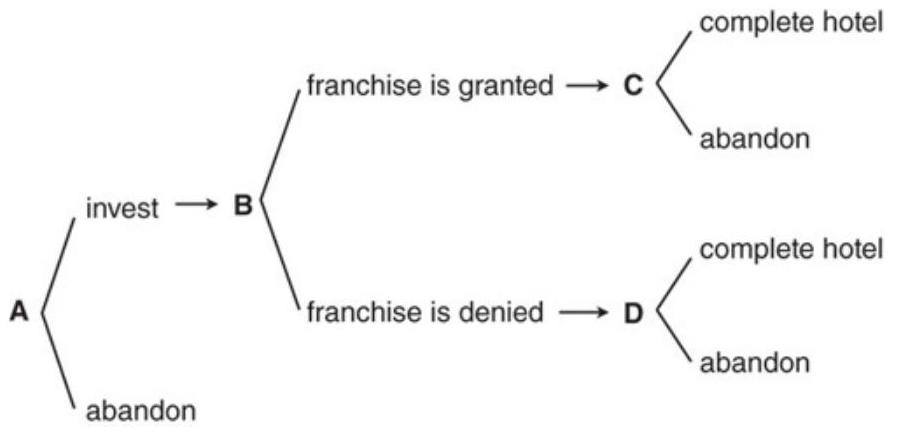
\includegraphics[max width=\textwidth]{2024_04_11_73a6b5609218251c8b58g-3(1)}
\end{center}

\section*{Decision Tree for the Sports Hotel}
The decision tree models two types of events: the arrival of new information and decisions. Alternative outcomes of decisions are illustrated vertically. Each potential decision is modeled as two or more branches that emanate from a decision node. The starting node in the exhibit above is labeled $A$ and represents a decision node. A decision node is a point in a decision tree at which the holder of the option must make a decision. In the case of node A, the decision is that the investor must decide whether to start the project. Node B represents an information node. An information node denotes a point in a decision tree at which new information arrives. In the case of node B, the information is the decision by the league as to whether a sports franchise will be granted.

\section*{Backward Induction and Decision Trees}
Backward induction is used to solve a problem involving options and using a decision tree. Backward induction is the process of solving a decision tree by working from the final nodes toward the first node, based on valuation analysis at each node. Backward induction guides the decision maker to resolve the final decisions first, since those decisions involve a single period and have no real options remaining unresolved. Then, working backward through time one period at a time, the decision maker can resolve decisions until the only remaining decision is the first one. Backward induction is also used in pricing financial derivatives.

The following exhibit illustrates backward induction. In the exhibit below, the ends of each path have been valued using the assumed information and based on all possible paths of outcomes and decisions; all uncertainty has been resolved. The analysis now moves to nodes $C$ and $D$, which are decision nodes representing points in time at which the investor can decide which path to take. The decisions of the investor at nodes $C$ and $D$ can be solved under the continuing and simplifying assumption that the appropriate discount rate is $0 \%$. For example, at node C, the investor would prefer to complete the hotel (receive $\$ 30$ million), and at node D, the investor would prefer to abandon the hotel (lose only $\$ 10$ million). These decisions are reflected in the exhibit, Sports Hotel Decision Tree with Final Decision Included. The process is repeated to value the project at node B, yielding a value of $\$ 10$ million (multiplying $\$ 30$ million by 0.5 and multiplying $-\$ 10$ million by 0.5 , and summing). The results are reflected in the exhibit, Sports Hotel Decision Tree with Final Decision and New Information Included.

\begin{center}
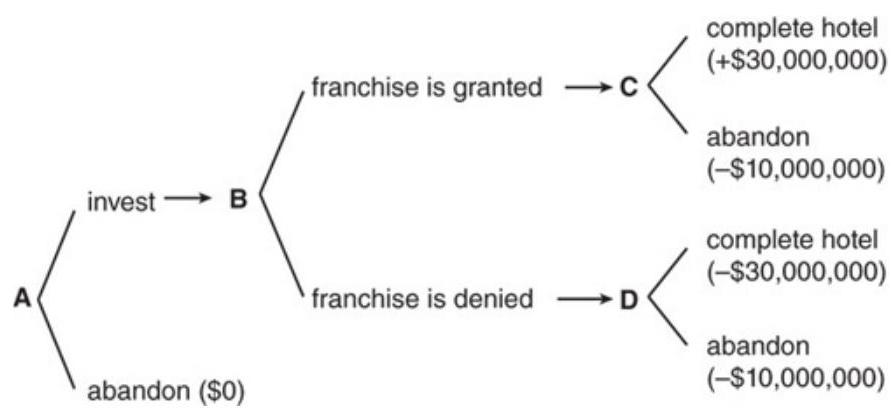
\includegraphics[max width=\textwidth]{2024_04_11_73a6b5609218251c8b58g-3}
\end{center}

The Sports Hotel Decision Tree with Final Nodes Value

\begin{center}
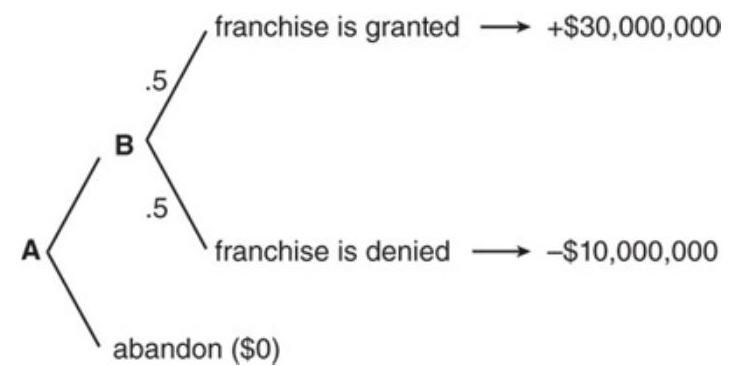
\includegraphics[max width=\textwidth]{2024_04_11_73a6b5609218251c8b58g-3(2)}
\end{center}

Sports Hotel Decision Tree with Final Decision Included

\begin{center}
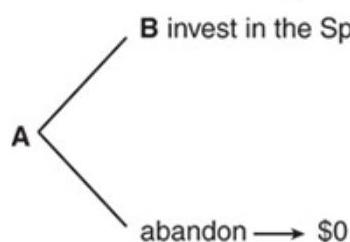
\includegraphics[max width=\textwidth]{2024_04_11_73a6b5609218251c8b58g-4}
\end{center}

\section*{Sports Hotel Decision Tree with Final Decision and New Information Included}
This above exhibit illustrates that the investor's decision is simple. Proceeding with the first-year plans for the hotel produces an expected profit of $\$ 10$ million. The project appeared to have no value, meaning expected benefits equaled expected costs, when options were ignored. However, when options are priced, the project has tremendous value. The essential driver of value emanating from an option analysis is the ability to revise plans when new information arrives. Real estate investment involves risk, and real estate development typically involves great risk. However, the risk that a developer might not be able to sell or lease when a real estate development is completed (e.g., because of adverse general market conditions) can be mitigated by preselling or preleasing all or part of the real estate development before its completion. Analysis using real options can help structure the problem such that the value of being able to defer decisions until after new information has arrived and uncertainty has been resolved can be assessed and appreciated.


\end{document}